\chapter{Test Cases}
\label{chap:landice_test_cases}

%Steve commented out line below because test case ARE currently available for download. 
%Eventually test cases will be available for download.  Currently they are only part of the Development code for MPAS-Land Ice.  

The test cases discussed below are available for download \href{http://mpas-dev.github.io/land_ice/download.html}{here}.

%% Steve added comment below, but then commented out, since Users do not have access to all of the code mentioned in
%% this quick start file (e.g., mesh gen. tools).
%For the test cases discussed below, additional information can be found in the detailed ``quick start" guide, found 
%\href{https://github.com/MPAS-Dev/MPAS-Documents/blob/master/landice/reference_manual/mpas_landice_quickstart.txt}{here}.

%%%All test cases can be downloaded from \url{http://mpas-dev.github.com}  The test cases for this version of the code are available at\\
%%%\url{http://mpas-dev.github.com/ocean/release_\version/release_\version.}.

\FloatBarrier

% ================================================================

\section{Halfar Dome}
\label{sec:halfar_description}
This test case describes the time evolution of a dome of ice as described by \citet{Halfar1983}.
This test provide an analytic solution for a flat-bedded SIA problem.

\begin{equation}
    \label{halfar}
    \frac{\partial H}{\partial t} = \nabla \cdot (\Gamma H^{n+2} |\nabla H|^{n-1} \nabla H)
\end{equation}
where $n$ is the exponent in the Glen flow law, commonly taken as 3, and $\Gamma$ is a positive constant:
\begin{equation}
    \Gamma = \frac{2}{n+2} A (\rho g)^n
\end{equation}

For $n=3$, this reduces to:
\begin{equation}
    H(t,r) = H_0 \left(\frac{t_0}{t}\right)^\frac{1}{9}  \left[ 1 - \left(  \left( \frac{t_0}{t} \right) ^ \frac{1}{18} \frac{r}{R_0} \right)^\frac{4}{3} \right] ^ \frac{3}{7}
\end{equation}
where
\begin{equation}
    t_0 = \frac{1}{18\Gamma} \left( \frac{7}{4} \right)^3 \frac{R_0^4}{H_0^7}
\end{equation}
and $H_0, R_0$ are the central height of the dome and its radius at time $t=t_0$.

For more details see \url{http://www.projects.science.uu.nl/iceclimate/karthaus/2009/more/lecturenotes/EdBueler.pdf},  \citet{Bueler2005}, \citet{Halfar1983}.



\subsection{Provided Files}
\label{subsec:halfar_files}
Our implementation of the Halfar dome has an initial radius of $R_0=21.2$ km and an initial thickness of $H=707.1$ m.
These values can be changed by editing \texttt{setup\_dome\_initial\_conditions.py}.

\begin{itemize}
	\item README: \\
		Information about the test case.

	\item namelist.landice: \\
		This file is used for actually running the dome test case in the MPAS land ice core.  It may not include all options available to the model.  See the namelist.landice.defaults file in the MPAS root directory for a list of all options available.  They are also documented in Section \ref{sec:forward_namelist_tables}.

	\item streams.landice: \\
		This file is used for specifying file input/output settings for the model.

	\item halfar.py: \\
		This is the script to compare model results to the analytic solution.

	\item visualize\_dome.py: \\
		This python script provides some general visualization of the model output.
		It can be used in addition to \texttt{halfar.py} for additional visualization.

%% Steve added comment below, but then commented out, since Users do not have access to grid gen tools.
%% Also, this file is no longer included in the tar archive of the test case.
%	\item namelist.input.periodic\_hex: \\
%		This file is used for running the grid generation tool \texttt{periodic\_hex} to create a grid for the test case.
%		It should be renamed to \texttt{namelist.input} when running the executable for \texttt{periodic\_hex}, which is
%		called \texttt{periodic\_grid}, and when run generates \texttt{grid.nc} \\
%		and \texttt{graph.info.part.*}.

%% Steve added comment below, but then commented out, since Users do not have access to grid gen tools
%	\item grid and initial condition files: \\ 
%		\texttt{grid.nc} is used as an input for \texttt{create\_landice\_grid\_from\_generic\_MPAS\_grid.py}, 
%%		located in \texttt{MPAS-Tools/grid\_gen/landice\_grid\_tools/}, 
%		which adds necessary initial condition data to the 	\texttt{grid.nc} file and renames it \texttt{landice\_grid.nc}. 
%		This file and the \texttt{graph.info.part.*} files can then be used as an input files when running the model 
%		on more than one processor.

	\item graph.info.part.* files: \\ 
		These provide grid partitioning information for running the test case on more than one processor.  
		
	\item setup\_dome\_initial\_conditions.py: \\
		This python script generates the dome initial condition after an empty \texttt{landice\_grid.nc} file exists.  
		If you downloaded a tar archive, you do not need to do this.  However, if you want to modify the IC for 
		some reason, you can edit and run this script.

\end{itemize}

\subsection{Results}
\label{subsecc:halfar_results}
As the dome of ice evolves, its margin advances and its thickness decreases (there is no surface mass balance to add new mass).  The script \texttt{halfar.py} will plot the modeled and analytic thickness at a specified time (Figure \ref{fig:halfarresults}), as well as report model error statistics.  Invoke \texttt{halfar.py --help} for details of its usage.


\begin{figure}[H!]
	\centering
	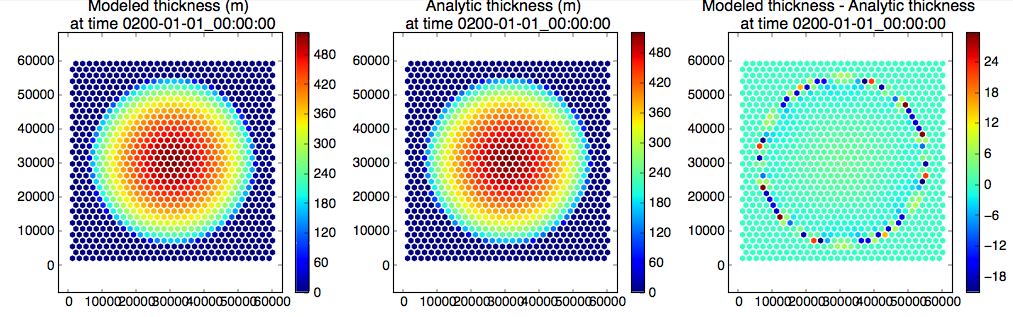
\includegraphics[width=16.4cm]{landice/figures/halfar.png}
	\caption{Halfar test case results after 200 years of dome evolution. This figure is generated by \texttt{halfar.py}.}
	\label{fig:halfarresults}
\end{figure}


\FloatBarrier

% ================================================================

\section{EISMINT-1 Test Cases}
\label{sec:eismint_description}
This test case is from the European Ice Sheet Modelling INiTiative intercomparison experiments.  These experiments are described at \url{http://homepages.vub.ac.be/~phuybrec/eismint.html} and in \citet{Huybrechts1996}.

Currently only the Moving Margin 1 Test Case from EISMINT-1 is included.


\subsection{Provided Files}
\label{subsec:eismint_files}


\begin{itemize}
\item namelist.landice: \\
	This file is used for actually running the dome test case in the MPAS land ice core.  It may not include all options available to the model.  See the namelist.landice.defaults file in the MPAS root directory for a list of all options available.  They are also documented in Section \ref{sec:forward_namelist_tables}.

\item streams.landice: \\
	This file is used for specifying file input/output settings for the model.

\item check\_output\_eismint-mm1.py \\
This script can be used to compare model output to results from the EISMINT intercomparison.

%% Steve added comment below, but then commented out, since Users do not have access to grid gen tools.
%% Also, this file is no longer included in the tar archive of the test case.
%\item namelist.input.periodic\_hex \\
% This file is used for running the grid generation tool \texttt{periodic\_hex} to create a grid for the test case.  It needs to be renamed to 'namelist.input' to run periodic\_hex) if mesh needs to be generated.  If you downloaded a tar archive of this test case, you do not need to create the mesh and can ignore this file.

\item graph.info.part.* files: \\ 
		These provide grid partitioning information for running the test case on more than one processor.  

\item setup\_initial\_conditions\_EISMINT1-MovingMargin-1.py \\
This file can be used to setup the initial conditions for the test case.  If you downloaded a tar archive, you do not need to do this.  However, if you want to modify the IC for some reason, you can edit and run this script.

\end{itemize}

\subsection{Results}
\label{subsecc:eismint_results}
As the initial ice sheet evolves, its shape eventually reaches a steady-state with the imposed surface mass balance.  
The script \texttt{check\_output\_eismint-mm1.py} will plot the modeled thickness at a specified time, 
as well as compare the model results to the results from the original EISMINT intercomparison.  
Invoke \texttt{check\_output\_eismint-mm1.py --help} for details of its usage.  
The script will compare the maximum ice thickness at the final time of the model output 
to the values reported from the models participating in the EISMINT-1 intercomparison.  
You should see something similar to this:

\begin{verbatim}
====================================
Max modeled thickness (m) = 2974.79474126
EISMINT models ice thickness at divide (m):
  3d models (10 of them): 2978.0 +/- 19.3
  2d models (3 of them):  2982.2 +/- 26.4
====================================
\end{verbatim}

% ================================================================


\section{Real World Test Cases}
Eventually grids for real-world Greenland and Antarctica will be provided at varying resolutions.


